% Chapter 2
\chapter{Efficient posterior sampling for Bayesian Poisson regression}
\chaptermark{Efficient posterior sampling for Poisson regression}


As we have seen in Section \ref{ch1_sec:spike_train_analysis}, encoding models are an important tool to study how the deconvolved spike trains vary with the underlying experimental conditions. To this end, GLMs provide a simple and flexible strategy to estimate the impact of each covariate on the mean of the variable of interest.
A relevant question that can be addressed using GLMs is how the number of spikes detected during a specific experiment is affected by the experimental conditions and the characteristics of the neurons. A plausible assumption to model the spike counts per time bin is to use a Poisson distribution~\citep{paninski2007}: in the context of GLMs, this setting naturally leads to the use of Poisson regression models. 

Poisson regression models are common in statistics and represent one of the most popular choices to model how the distribution of count data varies with predictors. A typical assumption is that, under an independent sample of counts, $y_1, \dots, y_n$, the probability mass function of the generic $y_i$ conditionally on a $p$-dimensional vector of covariates $x_i$ is
\begin{equation}
f(y_i \mid \lambda_i) =  \frac {\lambda_i^{y_i}}{{y_i}!}e^{-\lambda_i}, \quad \log(\lambda_i) = x_i^T \beta,
\label{ch2_eq:model0}
\end{equation}
where $\beta$ is a $p$-dimensional vector of unknown coefficients. Linking the linear predictor $x_i^T \beta$ and the parameter $\lambda_i$ with the logarithm represents the most natural choice, as the logarithm is the canonical link for the Poisson family~\citep{nelder1972glm}.
Besides encoding models for spike train analyses, this model has broad application in several fields, including medicine and epidemiology~\citep{Frome1983, frome1985, Hutchinson2005}, manufacturing process control~\citep{lambert1992}, analysis of accident rates~\citep{Sarath1990, Miaou1994}, and crowd counting~\citep{chan2009}, among others.

Adopting a Bayesian approach can be particularly convenient in the context of calcium imaging studies. As pointed out by \citet{paninski2007}, often some regularization technique is needed to obtain reliable estimates of the effects, as in some experiments the large number of covariates leads to a sensible risk of overfitting.
The Bayesian paradigm offers a natural approach to regularized regression: there is a large literature on prior inducing some kind of shrinkage or selection, as, for example, the spike-and-slab prior~\citep{mitchell1988}, the Bayesian lasso~\citep{park2008bayesian}, the horseshoe prior and its extensions \citep{carvalho2010horseshoe, Piironen2017}.

However, model \eqref{ch2_eq:model0} does not enjoy any conjugacy property and, thus, regardless of the prior used, the posterior distribution of $\beta$ is not available in close form. Consequently, inference is conducted using Markov Chain Monte Carlo (MCMC) methods, which obtain a sample from the posterior distribution of the parameters. Several approaches have focused on how to easily obtain the posterior distribution of the coefficients of Poisson models without requiring complex tuning strategies or long computation times. 
In the context of count-valued time series,~\cite{fruhwirth2006} proposed a formulation of the model based on two levels of data augmentation, to derive an efficient approximate Gibbs sampler. \cite{fruhwirth2009} exploited a data augmentation strategy to simplify the computation of hierarchical models for count and multinomial data.
Data augmentation strategies have also been employed in the case of models for multivariate dependent count data~\citep{karlis2005, bradley2018}. 
However, the simplest Poisson regression in \eqref{ch2_eq:model0} still lacks a specific and efficient algorithm to sample from the posterior distribution of the parameters $\beta$ for any prior choice, making the Metropolis-Hastings \citep{hastings1970monte} or Hamiltonian Monte Carlo (HMC) \citep{neal2011mcmc} algorithms the only available options.

On the other hand, several efficient computational strategies for binary regression models have been proposed in the literature. Using the probit link, \cite{albert_chib_1993} proposed an efficient data augmentation based on a latent Gaussian variable, while the more recent contribution by \cite{polson_scott_2013} exploited the canonical logit link, introducing an efficient P\'olya-gamma data augmentation scheme.
Leveraging \cite{polson_scott_2013} approach, we propose a novel approximation of the posterior distribution that can be exploited as proposal distribution of a Metropolis-Hastings algorithm or as importance density of an importance sampling for Poisson log-linear models with conditional Gaussian prior distributions on the regression parameters. With conditional Gaussian prior, we refer to a possibly hierarchical prior with conditional distribution $\beta \sim \mathrm{N}(b, B)$, with $b$ and/or $B$ random. Examples include straightforward Gaussian prior distributions with informative $(b,B)$ fixed using prior information, and scale mixtures of Gaussian where $b$ is set to zero and the variance has a suitable hierarchical representation, such as the Bayesian lasso prior or the horseshoe prior, among others.

More specifically, we introduce an approximation of the posterior density that exploits the negative binomial convergence to the Poisson distribution. Thanks to this result, we are able to leverage the P\'olya-gamma data augmentation scheme of~\cite{polson_scott_2013} to derive an efficient sampling scheme. 
In the next section, we introduce and discuss the proposed algorithms, starting from the definition of an \emph{approximate} posterior distribution whose sampling can be performed straightforwardly.
Sampling from this approximate posterior is then used as proposal density for the Metropolis-Hastings or importance sampler. The performance of the proposed algorithms in terms of computational efficiency is compared with that of state-of-the-art methods in a simulation study. Finally, we employ the proposed method to estimate a deconvolution model on spike train data from the Allen Brain Observatory.


\vfill

\section{Efficient posterior sampling strategies}
\label{ch2_sec:2}

\subsection{Approximate posterior distribution}\label{ch2_sec:approx_distr}

Assume $y_1,\dots,y_n$ is an independent sample of counts from model ~(\ref{ch2_eq:model0}). 
We introduce an approximation of the posterior density which exploits the negative binomial convergence to the Poisson distribution, i.e., we approximate the $i$-th contribution to the likelihood function $f(y_i \mid \lambda_i)$ with $\tilde{f}_{r_i}(y_i \mid \lambda_i)$ where 
\begin{equation}
\tilde{f}_{r_i}(y_i \mid \lambda_i) = \left( \frac{r_i}{r_i + \lambda_i}\right)^{r_i} \left(\frac{\lambda_i}{r_i+ \lambda_i}\right)^{y_i},
\label{ch2_eq:approx1}
\end{equation}
which corresponds to the probability mass function of a negative binomial random variable with parameter $r_i$, the number of failures until the experiment is stopped, and success probability $\lambda_i/(r_i+\lambda_i)$. As $r_i$ approaches infinity, this quantity converges to a Poisson likelihood.

Following \cite{polson_scott_2013}, we rewrite each $i$-th contribution to the approximate likelihood \eqref{ch2_eq:approx1} by introducing augmented P\'olya-gamma random variables $\omega_i \sim \mbox{PG}(y_i+r_i,0)$, i.e
\begin{align*}
\tilde{f}_{r_i}(y_i \mid \beta) = & \exp\left\{ \frac{(x_i^\T \beta - \log r_i)(y_i-r_i)}{2} \right\} 2^{-(y_i+r_i)} \times \\ 
& \int_{0}^{+\infty} \exp\left\{-\omega_i\frac{(x_i^\T \beta - \log r_i)^2}{2} \right\} \ppg(\omega_i; y_i + r_i,0) \, d\omega_i,   
\end{align*}
where $\ppg(\cdot; \xi,\zeta)$ denotes the density of a P\'olya-gamma with parameters $( \xi,\zeta)$. 
%

In what follows, we assume that prior knowledge about the unknown $\beta$ parameters is represented by a conditionally Gaussian prior, i.e. $\beta \sim \mathrm{N}(b, B)$, with a possible hierarchical representation for the parameters $b$ and $B$. Examples include default informative Gaussian with fixed $(b,B)$ or scale mixtures of Gaussian where $b$ is set to zero and the variance has a suitable hierarchical representation \citep{park2008bayesian, carvalho2010horseshoe, Piironen2017}.


The \emph{approximate} posterior based on the conditionally Gaussian prior $\beta \sim \mathrm{N}(b, B)$ and approximate likelihood $\prod_{i=1}^n \tilde{f}_{r_i}(y_i \mid \beta)$ is consistent with the successful Gibbs sampler of \cite{polson_scott_2013}; i.e., sampling from the \emph{approximate} posterior is equivalent to sampling iteratively from the following full conditionals 
\begin{equation}
\omega_i|\beta \sim \mbox{PG}(y_i + r_i, x_i^\T \beta - \log r_i), \qquad
\beta | y,\omega \sim \mathrm{N}_p(m_{\omega}, V_{\omega}),
\label{ch2_eq:approx0}
\end{equation}
where $V_{\omega} = (X^\T\Omega X + B^{-1})$ and $m_{\omega} = V_{\omega}(X^\T \kappa + B^{-1}b)$, with $\Omega = \mathrm{diag} \{\omega_1, \dots, \omega_n\}$ and $\kappa = (\omega_1 \log r_1 + (y_1-r_1)/2, \dots, \omega_n \log r_n + (y_n-r_n)/2)$.



The adherence of this approximate posterior to the true posterior highly depends on the values of $r_i$, with larger values of $r_i$ resulting in better approximations. However, when employing this result in posterior sampling, large values of $r_i$ imply longer computation time due to the computational cost of sampling P\'olya-gamma random variables with large parameters. Although the specific choice of $r_i$ remains an open point---discussed later in Section \ref{sec:tuning_param}---in the context of MCMC sampling, we propose to reduce the computational burden related to the sampling of $n$  P\'olya-gamma  random variables marginalizing the Gaussian distribution in \eqref{ch2_eq:approx0} with respect to the related P\'olya-gamma density conditioned on $\beta^{(t-1)}$,  the last available $\beta$ sampled. Since this marginalization is not in a closed form we introduce a second level of approximation of the true posterior. Specifically, we introduce $q(\beta \mid \beta^{(t-1)})$ a density that depends on $\beta^{(t-1)}$, defined as the first-order Taylor expansion of the marginalized Gaussian distribution, i.e. 
%\begin{align*}
%q(\beta\mid \beta^{(t-1)}) %&= \mathrm{E}_{\omega\mid\beta^{(t-1)}}\left\{ \phi(\beta\mid \omega_1,\dots,\omega_n) \right\}\\
%&=\mathrm{E}_{\omega\mid\beta^{(t-1)}} \left[ (2\pi)^{-p/2} \mathrm{det}(V_{\omega})^{-1/2} \exp\left\{-\frac{1}{2}(\beta - %m_{\omega})^\T V_{\omega} (\beta - m_{\omega})\right\} \right].
%\end{align*}
%Through a first order Taylor expansion we further obtain
\begin{equation}
\begin{aligned}
q(\beta\mid \beta^{(t-1)}) & = %\approx \phi(\beta\mid \mathrm{E}_{\omega\mid\beta^{(t-1)}}\left\{\omega_1\right\},\dots,\mathrm{E}_{\omega\mid\beta^{(t-1)}}\left\{\omega_n\right\})\\
%& \approx
(2\pi)^{-p/2} \mathrm{det}(V_{\mathrm{E}(\omega)})^{-1/2} \exp\left\{-\frac{1}{2}(\beta - m_{\mathrm{E}(\omega)})^\T V_{\mathrm{E}(\omega)}^{-1} (\beta - m_{\mathrm{E}(\omega)})\right\},
\end{aligned}
\label{ch2_eq:approx2}
\end{equation}
where $V_{\mathrm{E}(\omega)} = (X^\T \Omega X + B^{-1})$, $m_{\mathrm{E}(\omega)} = V_{\mathrm{E}(\omega)}(X^\T \kappa + B^{-1}b)$, 
$\Omega = \mathrm{diag} \{ \mathrm{E}(\omega_1),\dots,\mathrm{E}(\omega_n)\}$, $\kappa = (\mathrm{E}(\omega_1) \log r_i + (y_1-r_i)/2, \dots, \mathrm{E}(\omega_n) \log r_i + (y_n-r_i)/2)$, and for each $i = 1, \dots, n$ the conditional expectation of each $\omega_i$ is simply 
\begin{equation*}
\mathrm{E}\left(\omega_i^*\right) = \frac{r_i+y_i}{2(x_i^\T\beta^{(t-1)}-\log r_i)}\left(\frac{e^{x_i^\T\beta^{(t-1)}}-r_i}{e^{x_i^\T\beta^{(t-1)}}+r_i}\right),
\end{equation*}
or equivalently
\begin{equation}
\beta\mid \beta^{(t-1)} \sim \mathrm{N}(m_{\mathrm{E}(\omega)}, V_{\mathrm{E}(\omega)}).
\label{ch2_eq:proposal_distr}
\end{equation}
The above construction is eventually used as the building block of efficient Metropolis-Hastings and importance sampling algorithms, as described in the following sections.
%

\subsection{Metropolis-Hastings sampler}
\label{ch2_sec:mh}

We employ the above sampling mechanism as the proposal density in a Metropolis-Hastings algorithm. Consistent with this, at each iteration of the MCMC sampler, an additional step that accepts or rejects the proposed draw is introduced. Specifically, we assume that conditionally on the current state of the chain $\beta^{(t-1)}$, a new value $\beta^*$ is sampled from \eqref{ch2_eq:proposal_distr}. Then, the acceptance probability 
\begin{equation}
\alpha(\beta^*,\beta^{(t-1)}) = \min\left\{ 1, \frac{\pi(\beta^*\mid y)}{\pi(\beta^{(t-1)}\mid y)}\frac{q(\beta^{(t-1)}\mid \beta^*)}{q(\beta^{*}\mid \beta^{(t)})} \right\},
\label{ch2_eq:acceptanceMH}
\end{equation}
is evaluated to decide whether to accept or reject the proposed $\beta^*$, where $\pi(\beta^*\mid y)$ is the exact posterior distribution.

%
To compute the acceptance probability in \eqref{ch2_eq:acceptanceMH}, the forward and backward transition densities $q(\beta^*\mid \beta^{(t-1)})$ and $q(\beta^{(t-1)}\mid \beta^*)$ must be computed. Consistent with this,  approximation~(\ref{ch2_eq:approx2}) is particularly useful: without it, it would be necessary to compute the marginal density where the P\'olya-gamma random variables are integrated out. However, the marginalization with respect to the  P\'olya-gamma density does not lead to a closed form expression; thus, the Metropolis-Hastings algorithm cannot be defined. %For example, the density of $\beta^*$ conditioned on $\beta^{(t)}$ is
%\begin{equation}
%q(\beta^*\mid \beta^{(t)}) = \int_{\{\mathcal{R}^+\}^n} \phi(\beta^*\mid \omega_1^*,\dots,\omega_n^*)p(\omega_1^*,\dots,\omega_n^*\mid \beta^{(t)})d\omega_1^*\dots\omega_n^* 
%\label{ch2_eq:marginal}
%\end{equation} 
%where $\phi(\beta^*\mid \omega_1^*,\dots,\omega_n^*)$ is the density of $\beta^*$ conditioned on $\{\omega_1^*,\dots,\omega_n^*\}$, that is $\beta^*\mid\omega^*\sim N_p (m_{\omega^*}, V_{\omega^*})$, and $p(\omega_1^*,\dots,\omega_n^*\mid \beta^{(t)})$ is the density of $n$ independent $PG(r_i+y_i, x_i^\T\beta^{(t)}-\log r_i)$ random variables. 
%


%An analogous result holds for $q(\beta^{(t-1)}\mid \beta^{*})$, with the only difference that the expectation of the P\'olya-gamma random variables is conditioned on $\beta^*$ instead of $\beta^{(t-1)}$.
%Not only this Taylor approximation avoids the computation of the marginal density in~(\ref{ch2_eq:marginal}), but it also avoids the sampling the P\'olya-gamma random variables, as now the algorithm only involves Gaussian densities.
%

Clearly, for increasing $r_i$ the proposal density \eqref{ch2_eq:proposal_distr} is closer to the true full conditional distribution; hence, the related acceptance rate will be higher, and the Metropolis-Hastings algorithm will be similar to a Gibbs sampler. 
On the other hand, setting this parameter to get a lower acceptance rate can result in smaller autocorrelation, and hence a better mixing \citep{robert2010}. We discuss an approach to choose $r_i$ balancing these two extremes in Section~\ref{sec:tuning_param}.


\subsection{Adaptive importance sampler}
\label{ch2_sec:is}

The sampling mechanism \eqref{ch2_eq:proposal_distr} can also be exploited within the context of importance sampling, where the posterior expectation of a function of the parameter $\beta$, $\mathrm{E}\left( h(\beta) \right) = \int h(\beta)\, \pi(\beta \mid y) d\beta$ is evaluated via Monte Carlo integration without direct sampling from $\pi(\beta \mid y)$. To this end, the general approach is to define an importance density $q(\beta)$ that is used to sample values $\beta^{(1)}, \dots, \beta^{(T)}$, which are eventually averaged to obtain an approximation of $\mathrm{E}\left( h(\beta) \right)$ through
\[
\widehat{\mathrm{E}( h(\beta))} = \frac{1}{T} \sum_{t=1}^T \tilde{w}(\beta^{(t)}) h(\beta^{(t)}),
\]
with weights 
\begin{equation*}
\tilde{w}(\beta^{(t)}) = \frac{\pi(\beta^{(t)} \mid y)}{q(\beta^{(t)})}.
\end{equation*}
%Importance sampling can be also used when the target density $\pi$ is known up to a normalizing constant: in these cases it is sufficient to use the normalized version of the weights $w(\beta^{(t)}) = \tilde{w}(\beta^{(t)})/\bar{W}$ with $\bar{W} = T^{-1} \sum_{t=1}^T \tilde{w}(\beta^{(t)})$.

The efficiency of this algorithm is determined by the ability of the importance density to sample values relevant to the target density.
%: an estimate of the effective sample size of the obtained sample can be assessed through the quantity $\sum_{t=1}^T w(\beta^{(t)})^2 / (\sum_{t=1}^T w(\beta^{(t)}))^2$, which takes values between 1 and $n$~\citep{robert2010}.
To improve this aspect, we modify the original algorithm and, at each iteration, we simulate values from \eqref{ch2_eq:proposal_distr}, updating the importance density with \eqref{ch2_eq:approx2}. Thus, the importance density is adaptively updated based on the previously extracted value $\beta^{(t-1)}$ and the weights become
% . , hence $q(\beta^{(t)}) = q(\beta^{(t)}\mid \beta^{(t-1)})$.
\begin{equation*}
\tilde{w}(\beta^{(t)}) = \frac{\pi(\beta^{(t)} \mid y)}{q(\beta^{(t)} \mid \beta^{(t-1)})}.
\end{equation*}


\subsection{Tuning parameters $r_i$}
\label{sec:tuning_param}

The values of the parameters $r_i$, $i=1,\dots,n$, have to be tuned to balance the trade-off between acceptance rate and autocorrelation in the Metropolis-Hastings, and to control the mixing of the weights in the importance sampler. However, tuning $n$ parameters is not practical, especially for moderate to large $n$.
The first simple solution sets all  parameters equal to a single value $r$, however, in our experience, this resulted in a low effective sample size for some of the sampled chains.

As an alternative strategy, we choose to tune instead the distance of the proposal density from the target posterior.
As the expression of the posterior distribution is unknown, we control the distance between the Poisson and negative binomial likelihood. %: each $r_i$ is derived, conditionally on the last sampled $\beta^{(t)}$ and covariates $x_i$, to obtain a certain level of approximation. 
Based on \citet{Teerapabolarn2012}, we consider the upper bound of the relative error between the Poisson and negative binomial cumulative distribution functions. This result is particularly useful owing to its simplicity, which allows to analytically derive adequate parameters to bound the error to a specific value. Specifically, if $Y$ is a Poisson random variable with mean $\lambda_i$ and $V$ is a negative binomial random variable with parameters $r_i$ and $p_i$, as defined in Section~\ref{ch2_sec:approx_distr}, we have the following result:
\begin{equation*}
\mathrm{sup}_{y_i\geq 0} \left\lvert \frac{\mbox{Pr}(Y\leq y_i)}{\mbox{Pr}(V\leq y_i)} -1 \right\rvert = e^{-\lambda_i} p_i^{-r_i} - 1.
\end{equation*}

Hence, by setting an upper bound $d$ for the distance between the Poisson and negative binomial distribution, all the values of the parameters $r_i$ can be automatically derived to obtain a proposal density whose distance from the target posterior is constant for every $y_i$, even for heterogeneous data. Under our notation $p_i=\lambda_i/(r_i+\lambda_i)$, thus
$d = e^{-\lambda_i} ( 1 + r_i/\lambda_i)^{r_i} - 1,$
%\begin{equation*}
%    d = e^{-\lambda_i} \left( 1 + \frac{r_i}{\lambda_i} \right)^{r_i} - 1,
%\end{equation*}
which is solved by
\begin{equation}
r_i = - \lambda \log c \cdot
\left\{ \log c + \lambda \cdot\mathrm{W}\left( \frac{-c^{-1/\lambda} \log c}{\lambda} \right) \right\}^{-1},
\label{ch2_eq:r_solution}
\end{equation}
where $c=e^{\lambda}(d^2+1)$ and $\mathrm{W}(\cdot)$ is the Lambert-W function \citep{W}, which can be computed numerically using standard libraries. 
%
Hence, in the algorithm, at the beginning of each iteration, the values $r_1, \dots, r_n$ are computed according to~(\ref{ch2_eq:r_solution}) conditionally on the current value of $\beta$. %Then, these parameters are used to compute the mean and variance of the normal distribution~(\ref{ch2_eq:proposal_distr}) from which we extract a new proposed value for $\beta$.


\section{Numerical illustrations}
\label{ch2_sec:illustr}

\subsection{Synthetic data}
\label{ch2_sec:sim}

We conducted a simulation study under various settings to compare the efficiency of the proposed Metropolis-Hastings and importance sampler with that of state-of-the-art methods. We focused on the Hamiltonian Monte Carlo approach---as implemented in the Stan software \citep{stan}---as the successful Metropolis-Hastings with standard random walk proposal would require, different from the proposed approaches, the tuning of $p$ parameters, which becomes cumbersome for moderate to elevate $p$. The proposed methods are implemented via the R package \texttt{bpr}, %\citep{bpr}, 
which is written in efficient C++ language exploiting the \texttt{Rcpp} package \citep{RCPP} and available from the Comprehensive R Archive Network \citep{bpr} and in the repository
at \texttt{github.com/laura-dangelo/bpr}.

Data were generated from a Poisson log-linear model with sample sizes $n \in \{ 25, 50,$ $100, 200\}$ and number of covariates $p \in \{ 5, 10, 20\}$. 
Specifically, for each combination of $n$ and $p$, we consider 50 independent $n$ dimensional vectors of counts where each $y_i$ ($i = 1\dots, n$) is sampled from a Poisson distribution with mean $\lambda_i = e^{x_i^\T \beta}$, with common parameter $\beta$. The covariates were generated from continuous or discrete/categorical random variables under the constraints that the continuous variables have mean zero and variance one and that $1\leq \lambda_i \leq 200$. 

Two prior distributions for the coefficients $\beta$ were assumed, namely a vanilla Gaussian prior with independent components $\beta_j\sim \mathrm{N} (0,2)$, $j=1,\dots,p$, and the more complex horseshoe prior~\citep{carvalho2010horseshoe} which allows for the following  conditionally Gaussian representation
\begin{gather*}
\beta_j \mid \eta^2_j, \tau^2 \sim \mathrm{N}(0,\eta^2\tau^2) \\
\eta \sim \mathrm{C}^+(0,1), \quad \tau \sim \mathrm{C}^+(0,1),
\end{gather*}
for $j=1,\dots,p$, where $\mathrm{C}^+(0,1)$ is the standard half-Cauchy distribution. To implement the samplers under the horseshoe prior, we used the details of~\cite{makalic2016horseshoesampler}, and fixed the global shrinkage parameter $\tau$ to the ``optimal value'' $\tau_n(p_n) = (p_n/n)\sqrt{\log(n/p_n)}$, where $p_n$ is the number of non-zero parameters~\citep{vanderpas2017}. 

Each method introduced in Section \ref{ch2_sec:2}  was run for 10000 iterations with  5000 of them discarded as burn-in. The convergence of each algorithm was assessed by graphical inspection of the trace plots of the resulting chains. The convergence was satisfactory for all simulations and comparable for all algorithms, as no systematic bias was found in the posterior mean of the estimated parameters. 



To assess the efficiency of the proposed methods, we used a proxy of the time per independent sample, which is estimated as the total time (in seconds) necessary to simulate the entire chain, over the effective sample size of the resulting chain. For the proposed adaptive importance sampler, an estimate of the effective sample size was obtained using the quantity $\sum_{t=1}^T w(\beta^{(t)})^2 / (\sum_{t=1}^T w(\beta^{(t)}))^2$, which takes values between 1 and $n$~\citep{robert2010}. 
Notably, the burn-in samples were removed from the chains before computing the effective sample size. Thus, the obtained times per independent sample  do not represent exactly the number of seconds necessary to generate one independent sample---they rather represent an overestimate. Nonetheless, this approach provides a robust and fair comparison between the different competing algorithms. The experiment has been run on a Linux machine with 8 GB DDR4 2400 MHz RAM, CPU Intel i7-7700HQ 3.8 GHz, running R 4.1.1.
%
\begin{figure}[h]
	\begin{center}
		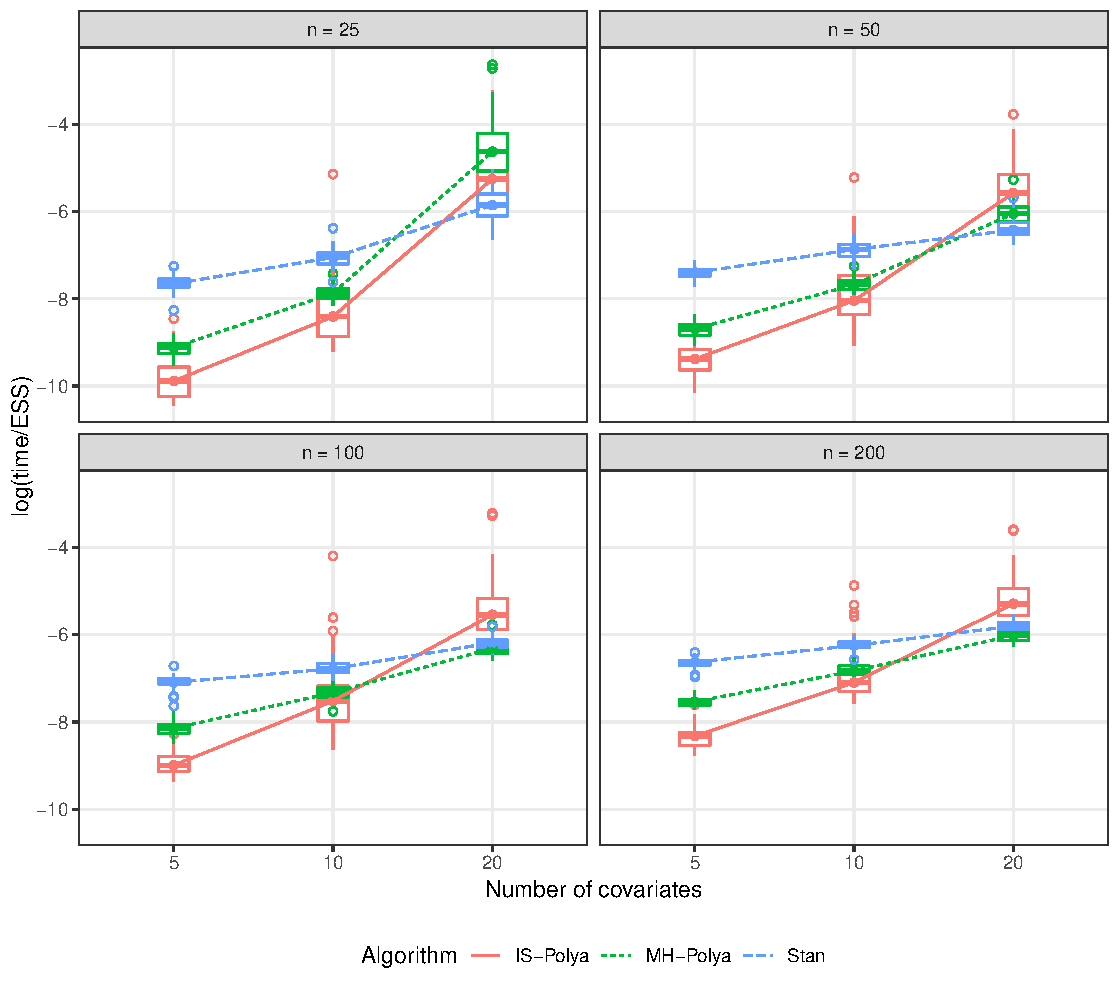
\includegraphics[width = .85\textwidth]{ch2_toess_gaussian.pdf}
		\caption[Comparison between the time per independent sample of the proposed algorithms and of the HMC algorithm.]{Time per independent sample (in logarithmic scale) for the three algorithms. For each combination of $n$ and $p$ the boxplots represent the distribution of the (log) time (in seconds) over the effective sample size using a Gaussian prior, over 50 replications.
		\label{fig:time_ess}}
	\end{center}
\end{figure}

Figure~\ref{fig:time_ess} and \ref{fig:time_ess_horseshoe} show, for each combination of $n$ and $p$, the distribution of the median time per independent sample for the three algorithms computed on the 50 replications under a Gaussian and horseshoe priors, respectively. The plots are presented in the logarithmic scale for clarity. 

For the Gaussian prior the performances of the proposed algorithms are better than those obtained using the HMC implemented in Stan, for small values of the dimension $p$. For $p=20$, instead, the performances of the HMC are quite competitive with respect to the importance sampling and broadly comparable to the proposed efficient Metropolis-Hastings algorithm. Notably, the differences are less evident with increasing sample size. 

\begin{figure}[h!]
	\begin{center}
		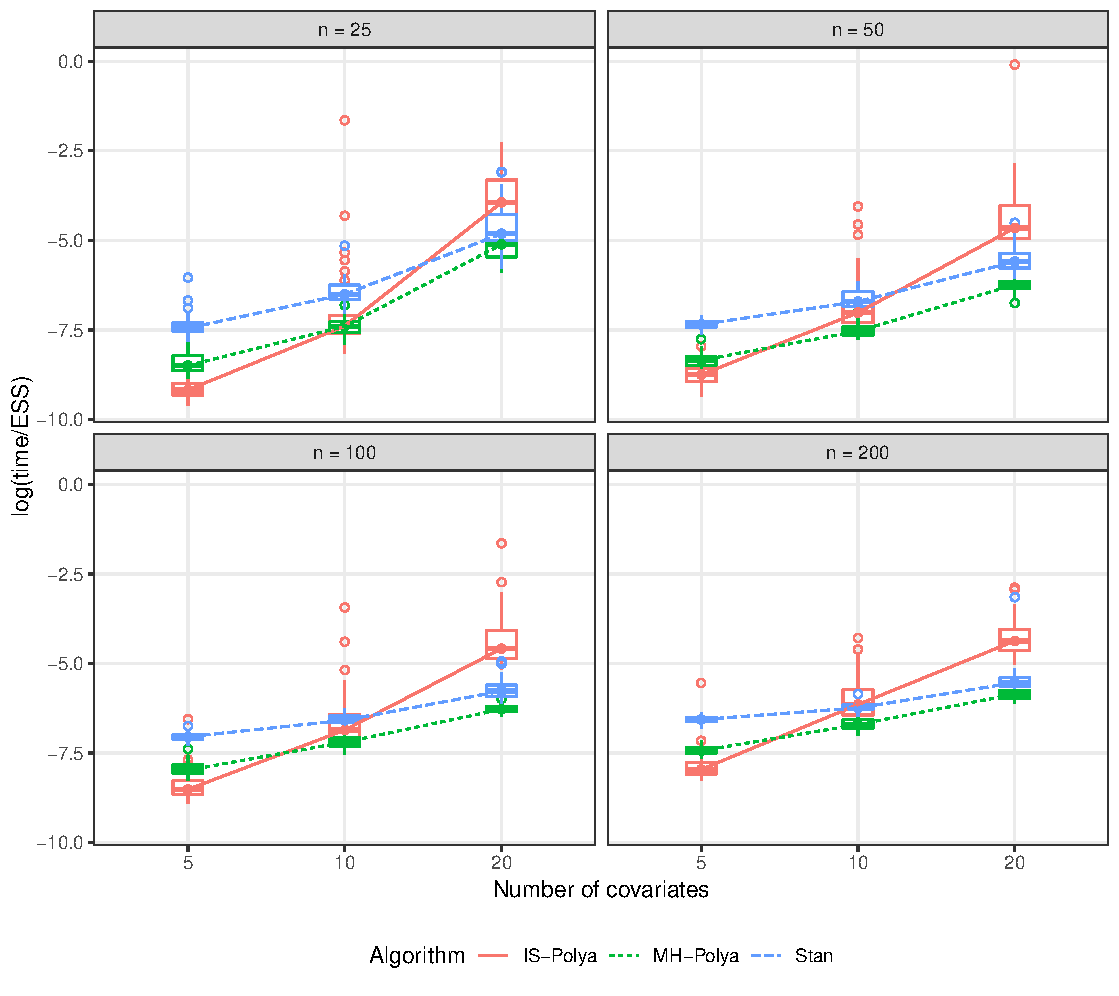
\includegraphics[width = .85\textwidth]{ch2_toess_horseshoe.pdf}
		\caption[Comparison between the time per independent sample of the proposed algorithms and of the HMC algorithm, using a horseshoe prior.]{Time per independent sample (in logarithmic scale) for the three algorithms. For each combination of $n$ and $p$ the boxplots represent the distribution of the (log) time (in seconds) over the effective sample size using the horseshoe prior, over 50 replications.
			\label{fig:time_ess_horseshoe}}
	\end{center}
\end{figure}
%
For the horseshoe prior, the proposed Metropolis-Hastings presents a stable superior performance with respect to the HMC sampler implemented in Stan for each sample size $n$ ad number of covariates $p$. The performance of the importance sampler remains competitive. As previously observed for the Gaussian prior, the differences are less evident for increasing sample size. 

%Hastings produces similar results to the HMC, with slightly better results for small $n$ and $p$. The use of a hierarchical prior mainly affects the importance sampler, which now has a lower efficiency compared to the other two approaches.




\subsection{Spike train data}
\label{ch2_sec:application}
%
Herein, we illustrate the proposed sampling method on data of brain activity in mice in response to visual stimulation.
The data set was generated using a small subset of data from the Allen Brain Observatory~\citep{allen}, described in detail in Section~\ref{ch1_sec:allen_brain_data}.
In the original data set, for each neuron the fluorescent calcium traces are recorded, which is a proxy of the neuronal activity, under different experimental conditions. From these traces, it is of interest to detect and analyze the activations of neurons, which correspond to transient spikes of the intracellular calcium level. 
We applied the method reported by~\citet{jewell2019} as described in~\citet{vries2020} to extract and count the activations of each neuron, to understand how they are affected by the experimental conditions and the location of the neurons in the brain. 

\begin{figure}[t]
	\centering
	\begin{subfigure}{\linewidth} \centering
		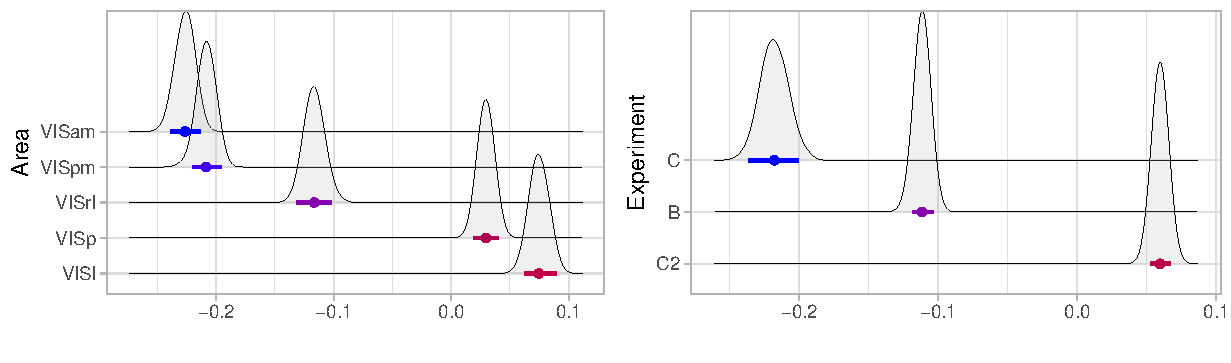
\includegraphics[width = \linewidth]{ch2_plot_area_exp.pdf}
	\end{subfigure}
	\begin{subfigure}{\linewidth} \centering
		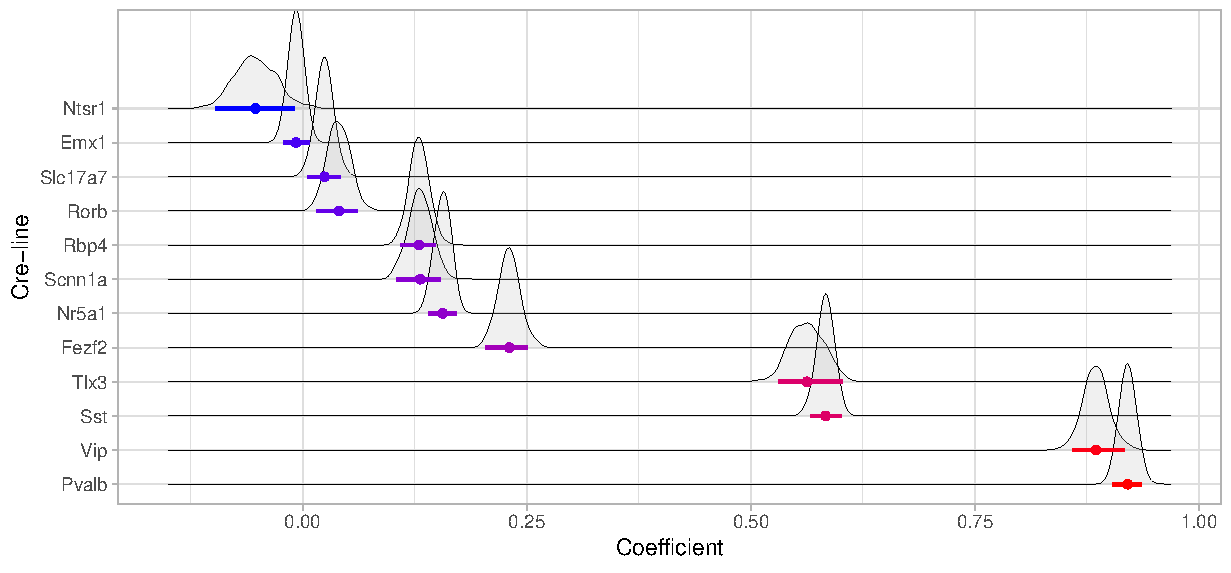
\includegraphics[width = \linewidth]{ch2_plot_cre.pdf}   \end{subfigure}
	\caption[Estimated coefficients of the regression on the calcium imaging data set.]{Estimated coefficients of the regression on the calcium imaging data set: posterior density, with the posterior mean and 95\% credible interval (colored dot and segment).} \label{fig:calcium_coeff}
\end{figure}


The covariates that we considered are the depth of the neuron, the area of the visual cortex where the neuron is located (factor with 6 levels), the cre transgenic mouse line (factor with 13 levels), and the type of visual stimulation (factor with 4 levels). 
The depth of the neurons is discretized to 22 levels, ranging from 175 to 625 microns, thus, we could obtain a data set having a full factorial design with 5 replications for each available covariate combination. Moreover, we included a quadratic term of the depth to improve the fitting. The obtained data set is made of 920 observations on 23 variables.


We ran the proposed Metropolis-Hastings algorithm for 9000 iterations, discarding the first 5000 as burn-in. The computation time was 98 seconds.
The posterior estimates of the coefficients of the dummies on three categorical variables are shown in Figure~\ref{fig:calcium_coeff}; and for the numeric covariate depth, the posterior mean and 95\% credible intervals were equal to $-2.72\times 10^{-3}$ $(-2.90\times 10^{-3}, -2.42\times 10^{-3})$ for the linear term, and $5.59\times 10^{-6}$ $(5.11\times 10^{-6}, 6.08\times 10^{-6})$ for the quadratic term.
Given these estimates of the coefficients, the number of spikes increased with the largest depths.
Moreover, as shown in Figure~\ref{fig:calcium_coeff}, the response of neurons is heterogeneous across the cre-lines and, coherent with the results of~\citet{vries2020}, we obtained that the mean response is lower for the VISam, VISpm and VISrl areas.

